% This file was created with tikzplotlib v0.9.12.
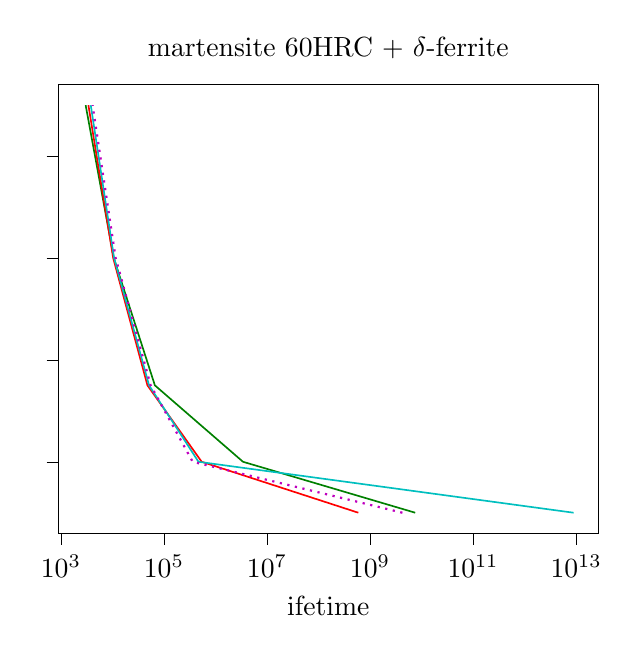
\begin{tikzpicture}

\definecolor{color0}{rgb}{0,0.75,0.75}
\definecolor{color1}{rgb}{0.75,0,0.75}
\definecolor{color2}{rgb}{0.75,0.75,0}

\begin{axis}[
legend cell align={left},
legend style={
  fill opacity=0.8,
  draw opacity=1,
  text opacity=1,
  at={(0.7,1.2)},
  anchor=south west,
  draw=white!80!black
},
log basis x={10},
tick align=outside,
tick pos=left,
title={martensite 60HRC + $\delta$-ferrite},
x grid style={white!69.0196078431373!black},
xlabel={ifetime},
xmin=897.982202455344, xmax=26750068072298.1,
xmode=log,
xtick style={color=black},
y grid style={white!69.0196078431373!black},
ylabel={},
ymin=460, ymax=1340,
ytick style={color=black},
yticklabels={}
]
%\addplot [semithick, blue]
%table {%
%	nan 500
%	nan 600
%	nan 750
%	nan 1000
%	nan 1300
%};
%\addlegendentry{0.0 \% Martensite mean}
\addplot [semithick, green!50!black]
table {%
	7539392038.19674 500
	3422841.21269617 600
	66736.5403746578 750
	10644.967975207 1000
	3023.04641436758 1300
};
%\addlegendentry{85.0 \% Martensite mean}
\addplot [semithick, red]
table {%
	593135205.113158 500
	540167.233016487 600
	47847.4724681349 750
	10348.0627102153 1000
	3420.96032001891 1300
};
%\addlegendentry{90.0 \% Martensite mean}
\addplot [semithick, color0]
table {%
	8937815473598.65 500
	467922.232691425 600
	51467.7956733226 750
	10770.9278431322 1000
	3800.40292038858 1300
};
%\addlegendentry{95.0 \% Martensite mean}
\addplot [thick, color1, dotted]
table {%
	4249519869.80768 500
	361507.391183297 600
	55227.855879268 750
	11542.3030161597 1000
	4116.77266814751 1300
};
%\addlegendentry{100.0 \% Martensite mean}
\end{axis}


\end{tikzpicture}
